\documentclass[12pt,a4paper]{extarticle}
\usepackage[margin=1in]{geometry}
\usepackage[slantfont,boldfont]{xeCJK}
\usepackage{graphicx}
\usepackage{caption}
\usepackage{float}
\usepackage{pgfplots}
\usepackage{subcaption}

\pgfplotsset{compat=1.12}
\setCJKmainfont{cwTeXKai}

\title{Machine Learning 2017 Spring\\Homework 3 Report}
\author{學號:\texttt{B03902048}\\系級:資工三\\姓名:林義聖}
\date{}

\begin{document}
\maketitle

\begin{enumerate}
	\item (1\%) 請說明你實作的 CNN model,其模型架構、訓練過程和準確率為何?
	\par 答:Figure \ref{fig:cnn-model-structure} 是我的 CNN model 的基本架構圖。這個模型的總參數數量為 6,746,215。部分細節無法完全呈現在上圖中,則一一列舉在下方:
  \begin{itemize}
    \item Validation:我將總數 28709 筆的訓練資料切成兩份,其中前 3000 筆為 validation 用,其餘的用來訓練模型。
    \item Image Pre-processing:我先將訓練模型用的資料,利用水平翻轉變成兩倍資料量(51418 筆),接著利用 Keras 的 ImageDataGenerator 來增加訓練資料。我使用了旋轉、水平位移、垂直位移、縮放和錯切(推移)。
    \item Normalization:我將所有資料的亮度範圍,從 0 到 255,縮放至 0 到 1 之間。
    \item ReLU layer:在所有 Convolution Layer 之後,我都接上 Leaky ReLU 來作 elementwise activation,並設定 $\alpha$ 為 0.05。在這之後,Convolution Layer 的輸出 x,會變成
    $$f(x) = \max(x, \alpha x)$$
    \item Batch Normalization:在所有 Activation Layer 之後(除了 output layer),我再接上 Batch Normalization Layer。如此一來,可以加快訓練過程的收斂速度,也可以避免 Overfitting。
    \item Optimizer:我使用 Adam 作為模型訓練的 Optimizer。
    \item Batch:我將 batch size 設定為 128。
  \end{itemize}

  \begin{figure}[ht]
    \centering
    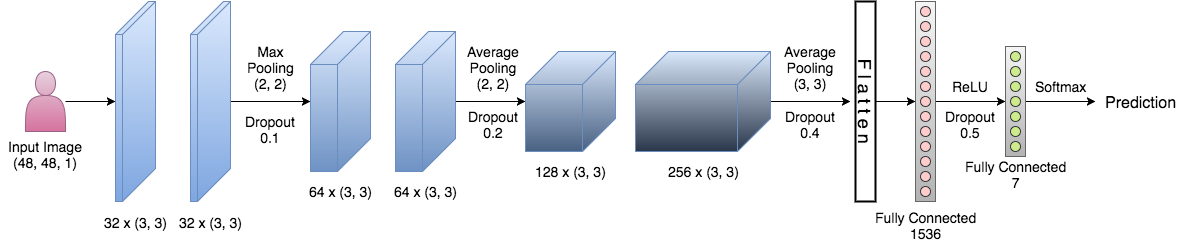
\includegraphics[width=0.9\linewidth]{cnn_model_structure.png}
    \caption{CNN model structure}
    \label{fig:cnn-model-structure}
  \end{figure}

  \par 訓練過程中,我一路將在 validation set 上有最高準確率的模型儲存下來,最終在 258 個 epochs 後,得到 0.7057 的準確率,而上傳之後,在 public set 上有 0.7127 的準確率。
  \par Figure \ref{fig:cnn-epoch-loss} 和 Figure \ref{fig:cnn-epoch-acc} 分別是訓練過程的 loss 和 prediciton accuracy 變化圖,根據這個分析表,我們可以看出,valid loss 在 10 到 20 個 epochs 間就開始上升,但是 valid accuracy 仍然可以在後續的訓練過程中,一點一點持續上升,我推測,這是做了 Image Pre-processing 帶來的效果。雖然隨著 valid loss 的上升,模型好像已經 overfit 在 training set 上,然而,透過 ImageDataGenerator,我們的訓練過程並沒有一筆完全固定的 training data,也因此,模型不至於 overfitting,所以可以在 validation set 上預測出好結果。

  \begin{figure}[ht]
    \begin{subfigure}[t]{0.5\textwidth}
    \begin{tikzpicture}
      \begin{axis}[
        xlabel = Epoch,
        legend pos = north east,
        ymajorgrids]
      \addplot[color=blue] table [x=epoch, y=loss, mark=none, col sep=comma] {cnn-training.csv};
      \addplot[color=red] table [x=epoch, y=valloss, mark=none, col sep=comma] {cnn-training.csv};
      \legend{training set,validation set}
      \end{axis}
    \end{tikzpicture}
    \caption{Cross-entropy loss}
    \label{fig:cnn-epoch-loss}
    \end{subfigure}
    \begin{subfigure}[t]{0.5\textwidth}
      \begin{tikzpicture}
        \begin{axis}[
          xlabel = Epoch,
          legend pos = south east,
          ymajorgrids]
        \addplot[color=blue] table [x=epoch, y=acc, mark=none, col sep=comma] {cnn-training.csv};
        \addplot[color=red] table [x=epoch, y=valacc, mark=none, col sep=comma] {cnn-training.csv};
        \legend{training set,validation set}
        \end{axis}
      \end{tikzpicture}
      \caption{Prediction accuracy}
      \label{fig:cnn-epoch-acc}
    \end{subfigure}
    \caption{CNN model training}
    \label{fig:cnn-training}
  \end{figure}

  \newpage

	\item (1\%) 承上題,請用與上述 CNN 接近的參數量,實做簡單的 DNN model。其模型架構、訓練過程和準確率為何?試與上題結果做比較,並說明你觀察到了什麼?
  \par 答:Figure \ref{fig:dnn-model-structure} 是我的 DNN model 的基本架構。這個模型的總參數數量為 6,581,255,與前一題的 CNN model 的 6,746,215 相去不遠。而這個 DNN model 的實作的細節,除了下方提及的 Activation Layer 和 Dropout 以外,其餘皆與前述的 CNN model 相同,好能比較他們之間的結果。

  \begin{figure}[ht]
    \centering
    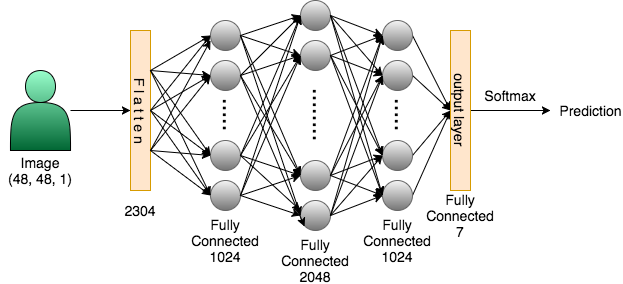
\includegraphics[width=0.9\linewidth]{dnn_model_structure.png}
    \caption{DNN model structure}
    \label{fig:dnn-model-structure}
  \end{figure}

  \begin{itemize}
    \item ReLU layer:在所有 hidden layer 之後,我都接上 ReLU 來作為 activation function。因此,前一層 hidden layer 的輸出 x 會變成
    $$f(x) = \max(0, x)$$
    \item Dropout:在 Figure \ref{fig:dnn-model-structure} 圖中的三層 hidden layer 之後,我分別加上 0.3, 0.4, 0.5 的 dropout。
  \end{itemize}

  \par 訓練過程中,我記錄了所有 training set 和 validation set 上的 loss 和 accuracy,最終在 399 個 epochs 的時候,在 validation set 上得到 0.4583 的準確率。Figure \ref{fig:dnn-epoch-loss} 和 Figure \ref{fig:dnn-epoch-acc} 分別是訓練過程的 loss 和 prediction accuracy 變化圖。

  \par 透過觀察這些變化圖,我們可以歸結兩個 DNN model 與 CNN model 不同的點:
  \begin{itemize}
    \item 在經過\textbf{相同回合數}後,我們可以明顯看出,DNN model 還沒有收斂,藉由 dropout,validation loss 仍顯著地低於 training loss,因此可以推測 model 還有相當大的進步空間。此外,雖然經過了相同數目的 epochs,DNN model 預測的準確率完全無法與 CNN model 相比,即使兩個模型的參數數量相近。經過這樣的比較,我們可以斷定,在表情辨識這個任務上,CNN model 明顯地優於 DNN model,不僅能收斂地更快,也能達到更高的準確度。值得一提的是,DNN model 的訓練相對的快,可以花大約一半的時間,便達到同樣數目的 epochs。

    \item \textbf{繼續訓練}這個模型,達到 650 epochs 後,這時的訓練時間已經與 CNN model 相去不遠,然而,DNN model 的訓練還沒收斂,看起來仍有不小的進步空間。透過觀察 Figure \ref{fig:dnn-training-650},我們可以發現,它相較於 Figure \ref{fig:dnn-training} 中的曲線,幾乎沒有明顯改變,因此可以推斷,DNN model 要達到收斂,可能要再花上相當長的時間。所以,即使 DNN model 仍有進步的空間,要訓練好它所花的時間早已遠超 CNN model,且未必能達到更高的準確度。
  \end{itemize}

  \begin{figure}[H]
    \begin{subfigure}[t]{.5\textwidth}
      \begin{tikzpicture}
        \begin{axis}[
          xlabel = Epoch,
          legend pos = north east,
          ymajorgrids]
        \addplot[color=blue] table [x=epoch, y=loss, mark=none, col sep=comma] {dnn-training.csv};
        \addplot[color=red] table [x=epoch, y=valloss, mark=none, col sep=comma] {dnn-training.csv};
        \legend{training set,validation set}
        \end{axis}
      \end{tikzpicture}
      \caption{Cross-entropy loss}
      \label{fig:dnn-epoch-loss}
    \end{subfigure}
    \begin{subfigure}[t]{.5\textwidth}
      \begin{tikzpicture}
        \begin{axis}[
          xlabel = Epoch,
          legend pos = south east,
          ymajorgrids]
        \addplot[color=blue] table [x=epoch, y=acc, mark=none, col sep=comma] {dnn-training.csv};
        \addplot[color=red] table [x=epoch, y=valacc, mark=none, col sep=comma] {dnn-training.csv};
        \legend{training set,validation set}
        \end{axis}
      \end{tikzpicture}
      \caption{Prediction accuracy}
      \label{fig:dnn-epoch-acc}
    \end{subfigure}
    \caption{DNN model training}
    \label{fig:dnn-training}
  \end{figure}

  \begin{figure}[H]
    \begin{subfigure}[t]{.5\textwidth}
      \begin{tikzpicture}
        \begin{axis}[
          xlabel = Epoch,
          legend pos = north east,
          ymajorgrids]
        \addplot[color=blue] table [x=epoch, y=loss, mark=none, col sep=comma] {dnn-training-650.csv};
        \addplot[color=red] table [x=epoch, y=valloss, mark=none, col sep=comma] {dnn-training-650.csv};
        \legend{training set,validation set}
        \end{axis}
      \end{tikzpicture}
      \caption{Cross-entropy loss}
      \label{fig:dnn-epoch-loss-650}
    \end{subfigure}
    \begin{subfigure}[t]{.5\textwidth}
      \begin{tikzpicture}
        \begin{axis}[
          xlabel = Epoch,
          legend pos = south east,
          ymajorgrids]
        \addplot[color=blue] table [x=epoch, y=acc, mark=none, col sep=comma] {dnn-training-650.csv};
        \addplot[color=red] table [x=epoch, y=valacc, mark=none, col sep=comma] {dnn-training-650.csv};
        \legend{training set,validation set}
        \end{axis}
      \end{tikzpicture}
      \caption{Prediction accuracy}
      \label{fig:dnn-epoch-acc-650}
    \end{subfigure}
    \caption{DNN model training to 650 epochs}
    \label{fig:dnn-training-650}
  \end{figure}

  \newpage

	\item (1\%) 觀察答錯的圖片中,哪些 class 彼此間容易用混?(繪出 confusion matrix 分析)
	\par 答:我使用 sklearn 套件當中的 \texttt{confusion\_matrix} 函式來算出 confusion matrix,並繪製出 Figure \ref{fig:confusioin-matrix}。

  \begin{figure}[ht]
    \centering
    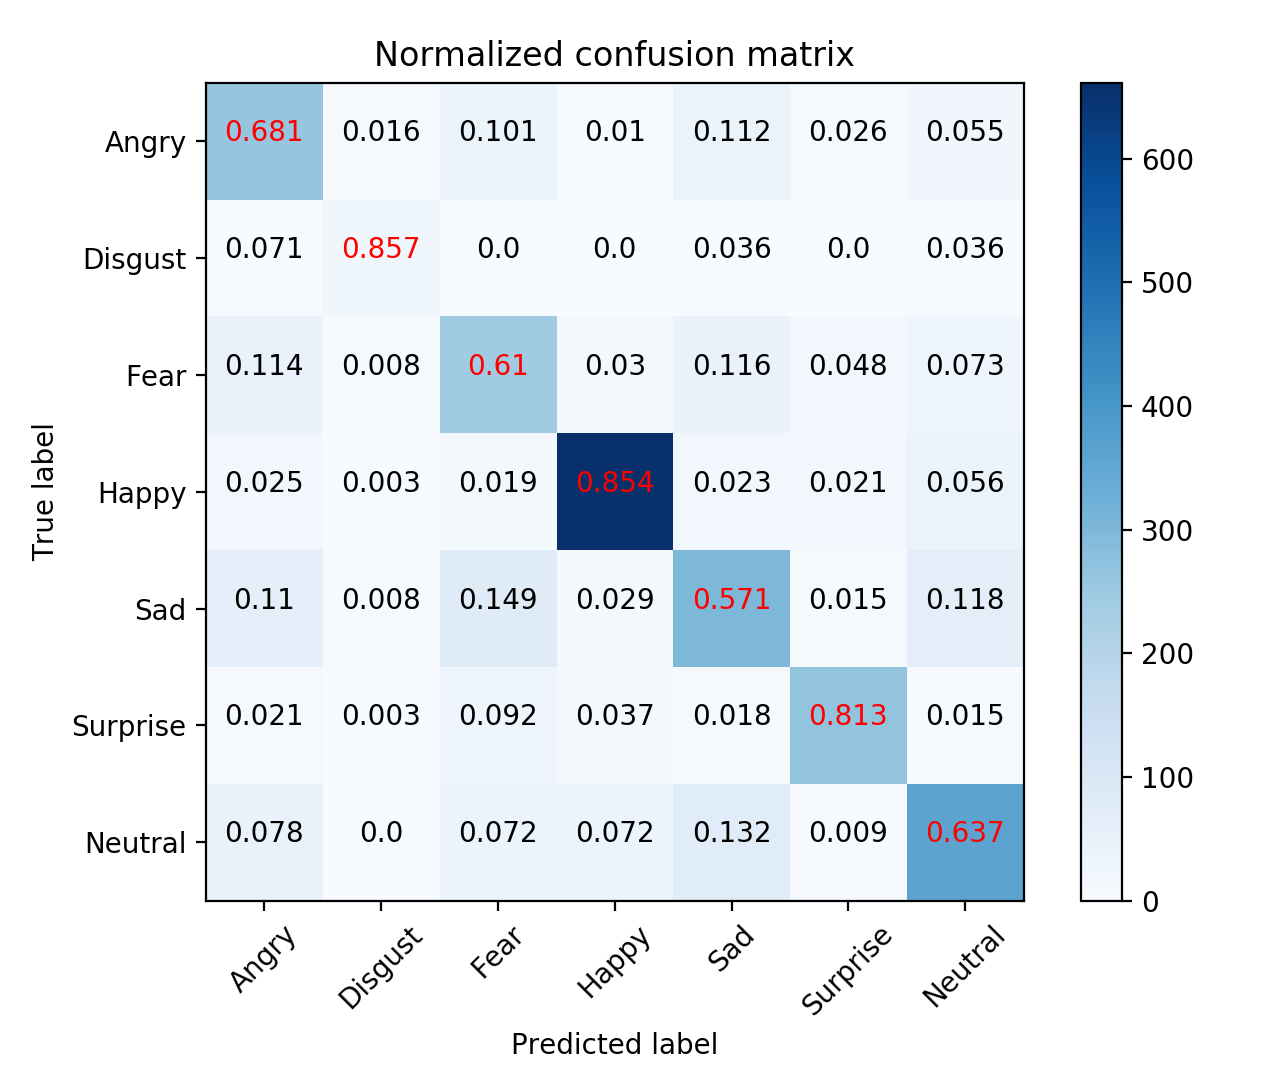
\includegraphics[width=\linewidth]{conf_mat_normalized.png}
    \caption{Normalized Confusion Matrix}
    \label{fig:confusioin-matrix}
  \end{figure}

  \par 觀察 confusion matrix 候,可以發現表情 Sad 和 Fear 之間,以及 Sad 和 Neutral 之間都很容易預測錯誤。先以 Sad 和 Fear 為例,以下有兩張來自 training set 的圖片,其中 Figure \ref{fig:train-image-2} 被預測成 Sad,然而它的標記其實是 Fear;而 Figure \ref{fig:train-image-6} 被預測成 Fear,然而它的標記其實是 Sad。

  \begin{figure}[ht]
    \begin{subfigure}[t]{0.5\textwidth}
      \centering
      
\includegraphics[width=0.8\linewidth]{train-image-2.png}
      \caption{Predicted as ``Sad''}
      \label{fig:train-image-2}
    \end{subfigure}
    \begin{subfigure}[t]{0.5\textwidth}
      \centering
      
\includegraphics[width=0.8\linewidth]{train-image-6.png}
      \caption{Predicted as ``Fear''}
      \label{fig:train-image-6}
    \end{subfigure}
    \caption{Misprediction between class ``Sad'' and ``Fear''}
    \label{fig:misprediction}
  \end{figure}

  \par 我認為 Figure \ref{fig:train-image-2} 是很容易誤判的,連我認為它是屬於 ``Sad''。至於 Figure \ref{fig:train-image-6},我覺得也不容易判斷,難以斷定是屬於 Sad 還是 Fear。而 Table \ref{tab:prob-distribution} 是 model 判斷出的那兩張圖片表情的機率分佈,從這個分佈,也可清楚看出,人容易搞混的圖片,model 也難以精確地做判斷。

  \begin{table}[ht]
    \centering
    \caption{Probability distribution}
    \label{tab:prob-distribution}
    \begin{tabular}{|c|c|c|c|c|c|c|c|}\hline
    \# & Angry & Disgust & Fear & Happy & Sad & Surprice & Neutral \\\hline
    Figure \ref{fig:train-image-2} & 0.06 & 0 & 0.07 & 0 & 0.87 & 0 & 0 \\\hline
    Figure \ref{fig:train-image-6} & 0 & 0 & 0.48 & 0 & 0.44 & 0 & 0.08 \\\hline
    \end{tabular}
  \end{table}

  \newpage

	\item (1\%) 從(1)(2)可以發現,使用 CNN 的確有些好處,試繪出其 saliency maps,觀察模型在做 classification 時,是 focus 在圖片的哪些部份?
	\par 答:我從 \texttt{train.csv} 裡面的前 3000 筆資料當中,選了第 11, 15 和第 30 張圖片來繪製 saliency maps,分別是 Figure \ref{fig:image-10-comparison}, Figure \ref{fig:image-14-comparison} 和 Figure \ref{fig:image-29-comparison}。
  \par 首先,Figure \ref{fig:image-10-comparison} 是一張標記為``生氣''的表情。所以,我認為判斷的重點在雙眼附近的皺紋,而 Figure \ref{fig:heatmap-10} 中的 heatmap 上高亮的區域正是那裡。而 Figure \ref{fig:image-14-comparison} 是一張標記為``快樂''的圖片。我認為判斷的重點是雙眼,以及嘴角的弧度,顯然地,從 Figure \ref{fig:partial-14} 來看,model 抓到的重點與我的判斷非常相像。最後,Figure \ref{fig:image-29-comparison} 是一張標記為``驚訝''的圖片。明顯地,瞪大的雙眼和大開的嘴巴是我們判斷的依據,而 Figure \ref{fig:partial-29} 中也清楚地顯示了模型是 focus 在這個部分。

  \begin{figure}[ht]
    \begin{subfigure}[t]{0.32\textwidth}
      \centering
      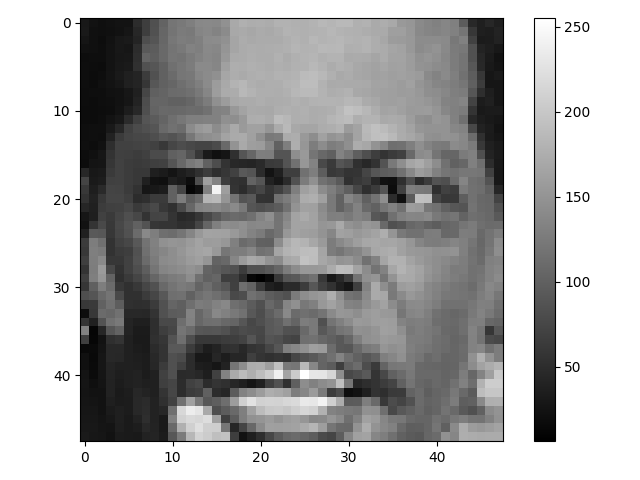
\includegraphics[width=\linewidth]{origin-10.png}
      \caption{Origin image}
      \label{fig:origin-10}
    \end{subfigure}
    \begin{subfigure}[t]{0.32\textwidth}
      \centering
      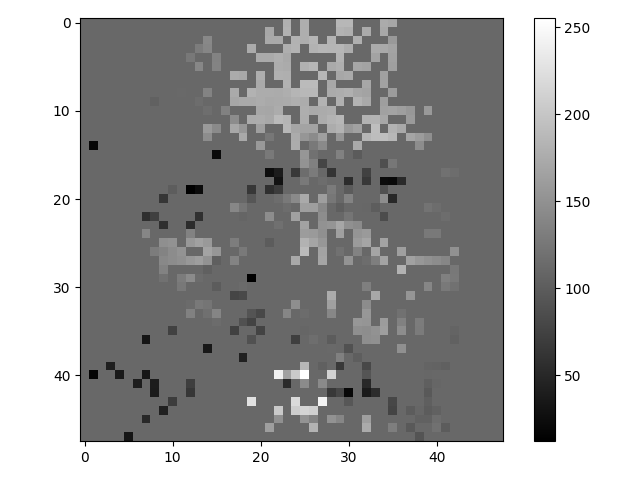
\includegraphics[width=\linewidth]{partial-10.png}
      \caption{Partial see}
      \label{fig:partial-10}
    \end{subfigure}
    \begin{subfigure}[t]{0.32\textwidth}
      \centering
      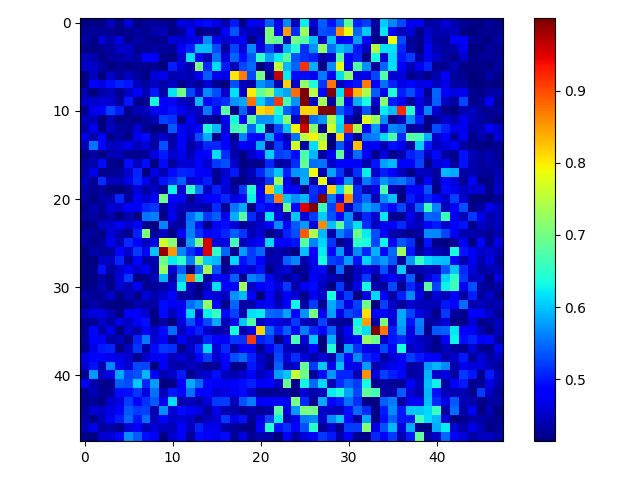
\includegraphics[width=\linewidth]{heatmap-10.png}
      \caption{Heatmap}
      \label{fig:heatmap-10}
    \end{subfigure}
    \caption{An ``Angry'' image in train.csv}
    \label{fig:image-10-comparison}
  \end{figure}

  \begin{figure}[ht]
    \begin{subfigure}[t]{0.32\textwidth}
      \centering
      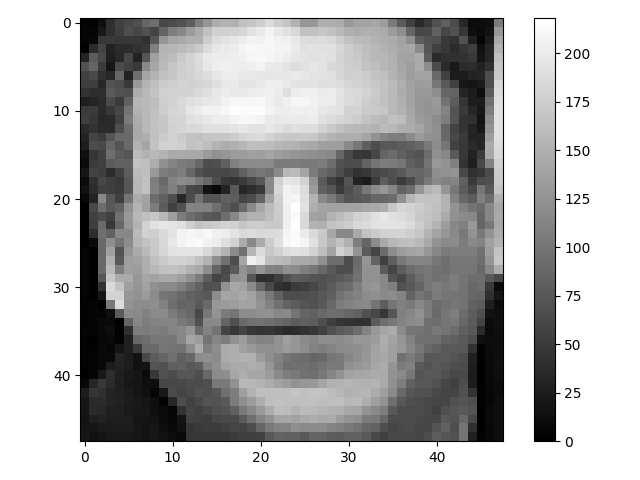
\includegraphics[width=\linewidth]{origin-14.png}
      \caption{Origin image}
      \label{fig:origin-14}
    \end{subfigure}
    \begin{subfigure}[t]{0.32\textwidth}
      \centering
      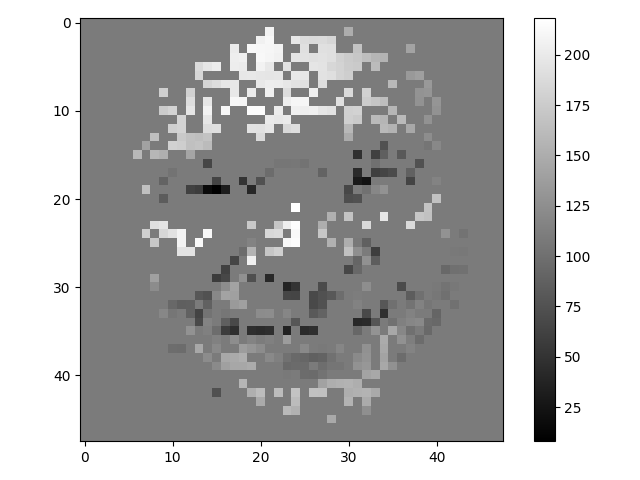
\includegraphics[width=\linewidth]{partial-14.png}
      \caption{Partial see}
      \label{fig:partial-14}
    \end{subfigure}
    \begin{subfigure}[t]{0.32\textwidth}
      \centering
      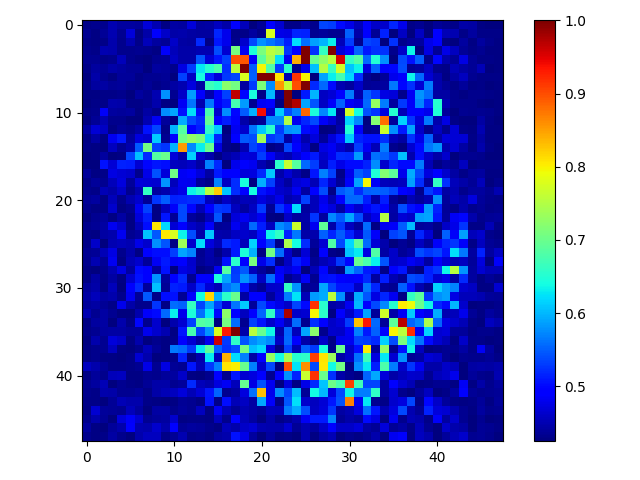
\includegraphics[width=\linewidth]{heatmap-14.png}
      \caption{Heatmap}
      \label{fig:heatmap-14}
    \end{subfigure}
    \caption{A ``Happy'' image in train.csv}
    \label{fig:image-14-comparison}
  \end{figure}

  \begin{figure}[ht]
    \begin{subfigure}[t]{0.32\textwidth}
      \centering
      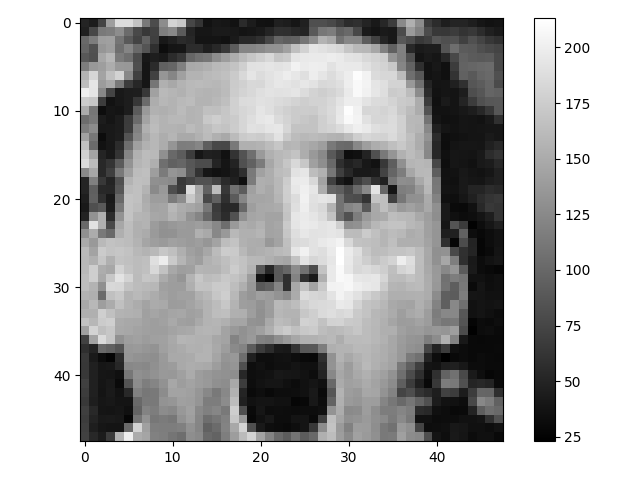
\includegraphics[width=\linewidth]{origin-29.png}
      \caption{Origin image}
      \label{fig:origin-29}
    \end{subfigure}
    \begin{subfigure}[t]{0.32\textwidth}
      \centering
      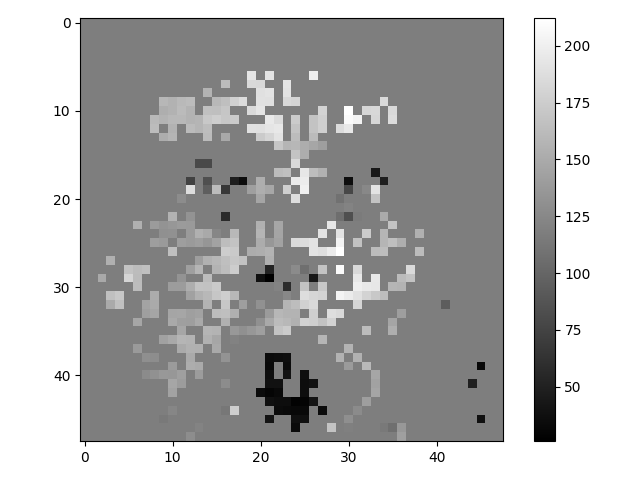
\includegraphics[width=\linewidth]{partial-29.png}
      \caption{Partial see}
      \label{fig:partial-29}
    \end{subfigure}
    \begin{subfigure}[t]{0.32\textwidth}
      \centering
      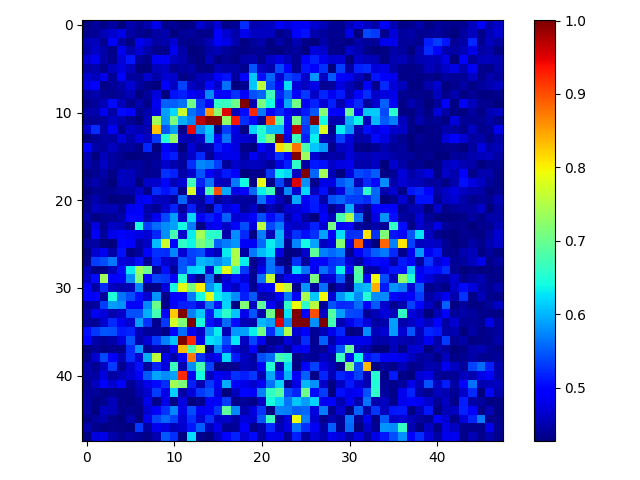
\includegraphics[width=\linewidth]{heatmap-29.png}
      \caption{Heatmap}
      \label{fig:heatmap-29}
    \end{subfigure}
    \caption{A ``Surprise'' image in train.csv}
    \label{fig:image-29-comparison}
  \end{figure}

  \newpage

	\item (1\%) 承(1)(2),利用上課所提到的 gradient ascent 方法,觀察特定層的 filter 最容易被哪種圖片 activate。
	\par 答:首先是 Figure \ref{fig:ga-white-noise},這整組圖片都是透過 gradient ascent 得到最容易激活 Leaky ReLU Layer 的圖片。我們可以觀察到,從 Figure \ref{fig:leaky_relu_1_e60} 上,也就是第一層當中,大多數圖片紋理都比較粗糙。也就是說,底層的 filter,基本上是在抓取圖片當中臉部的輪廓。而到了較上層的 filter,也就是在 Figure \ref{fig:leaky_relu_4_e60} 中,已經可以看到一些很重要的臉部特徵,如:眼睛、耳朵和皺紋等等。

  \begin{figure}[H]
    \begin{subfigure}[t]{0.5\textwidth}
      \centering
      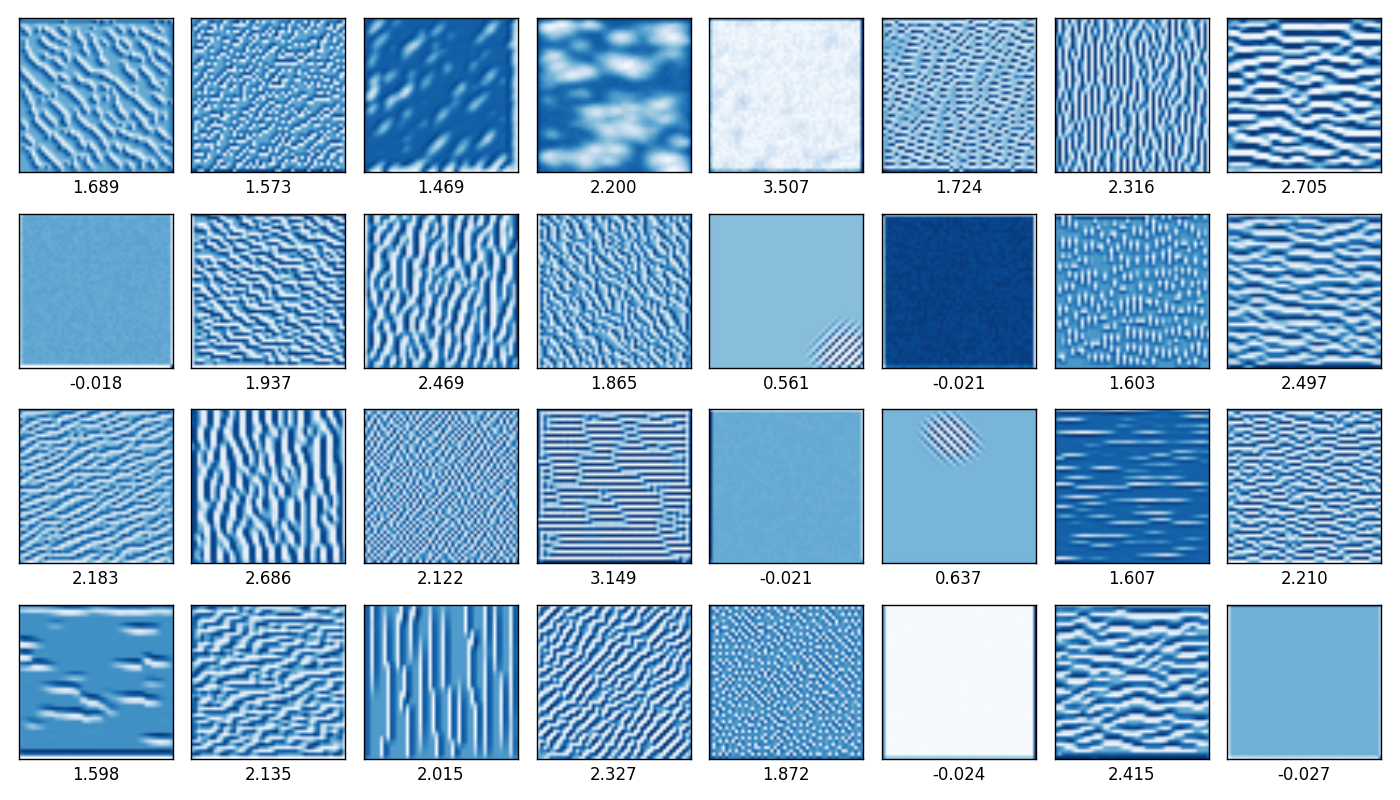
\includegraphics[width=\linewidth]{leaky_re_lu_1_e60.png}
      \caption{Layer: leaky relu 1 (epoch 60)}
      \label{fig:leaky_relu_1_e60}
    \end{subfigure}
    \begin{subfigure}[t]{0.5\textwidth}
      \centering
      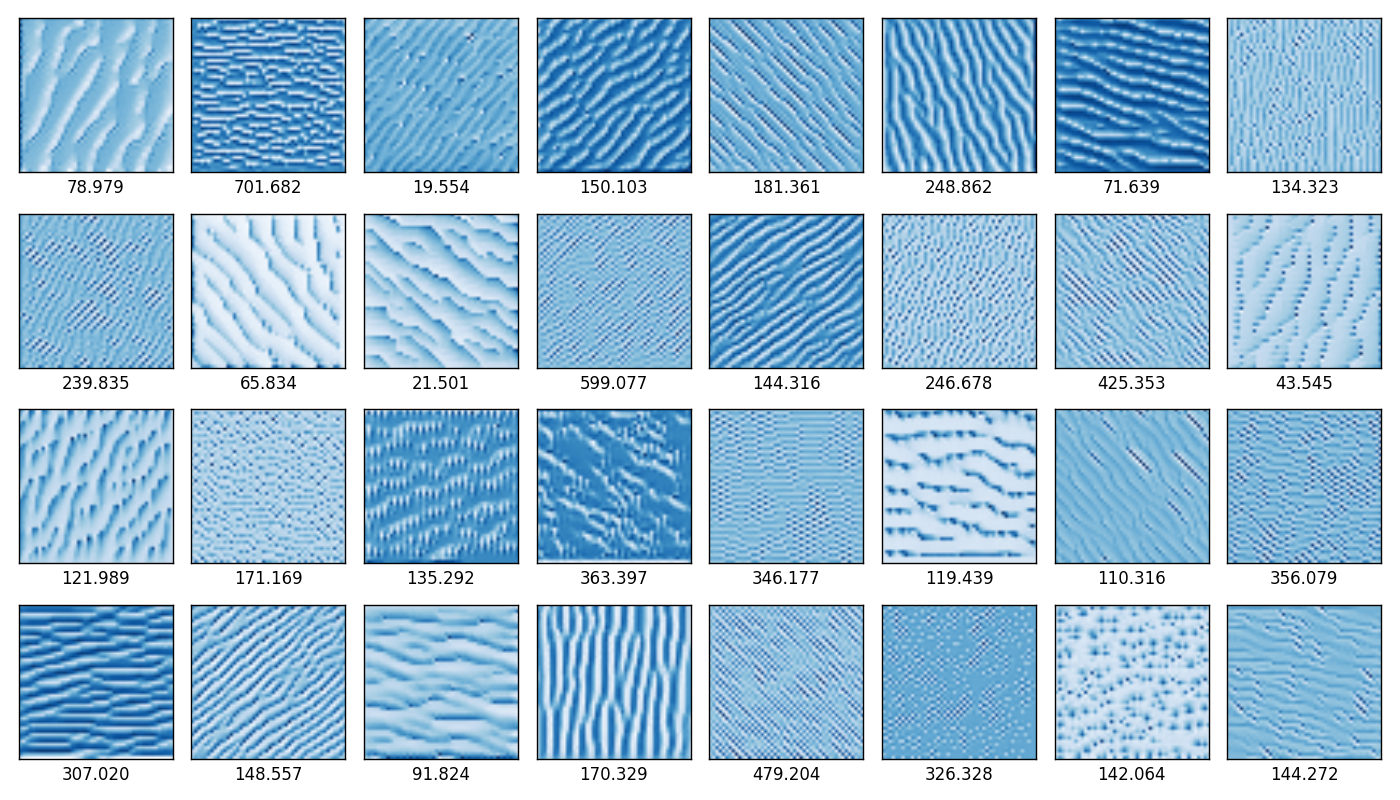
\includegraphics[width=\linewidth]{leaky_re_lu_2_e60.png}
      \caption{Layer: leaky relu 2 (epoch 60)}
      \label{fig:leaky_relu_2_e60}
    \end{subfigure}
    \begin{subfigure}[t]{0.5\textwidth}
      \centering
      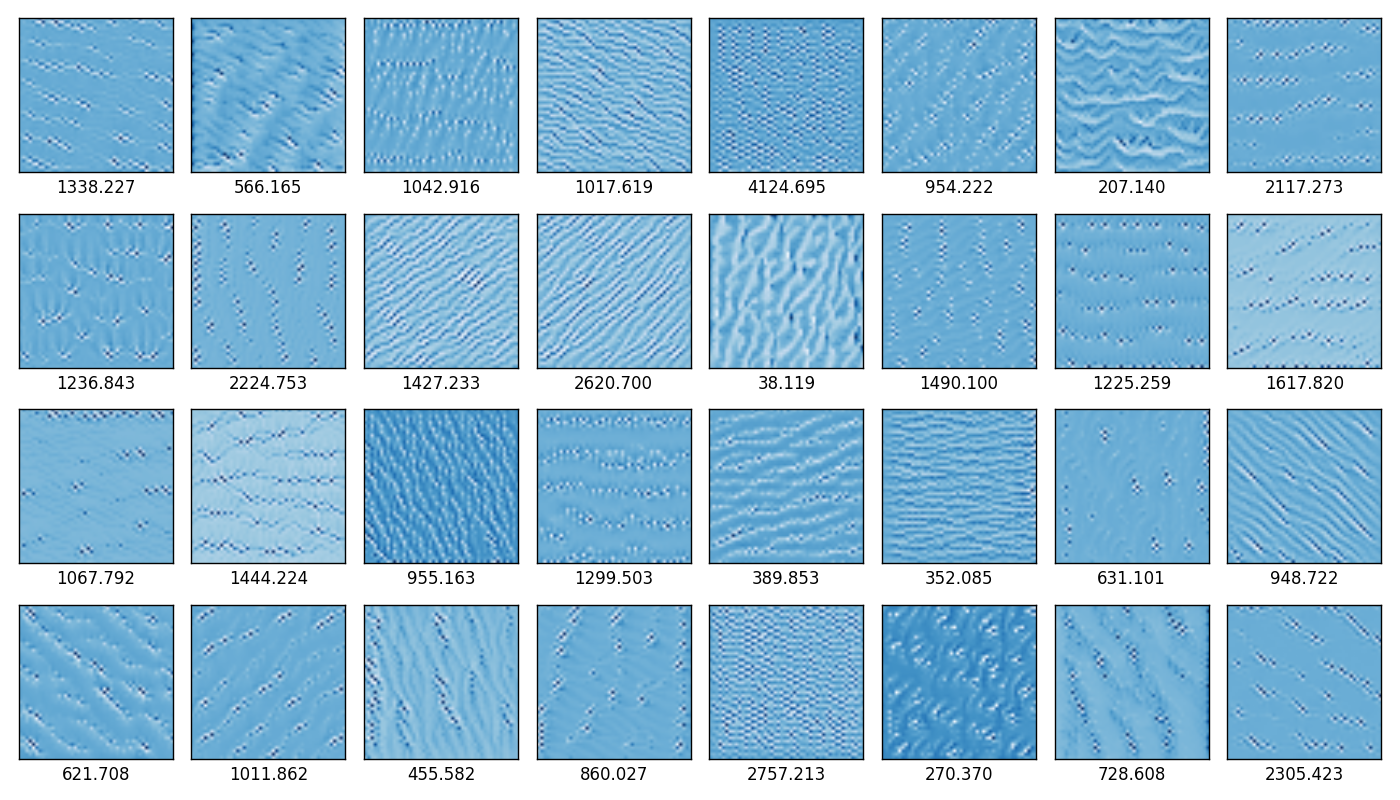
\includegraphics[width=\linewidth]{leaky_re_lu_3_e60.png}
      \caption{Layer: leaky relu 3 (epoch 60)}
      \label{fig:leaky_relu_3_e60}
    \end{subfigure}
    \begin{subfigure}[t]{0.5\textwidth}
      \centering
      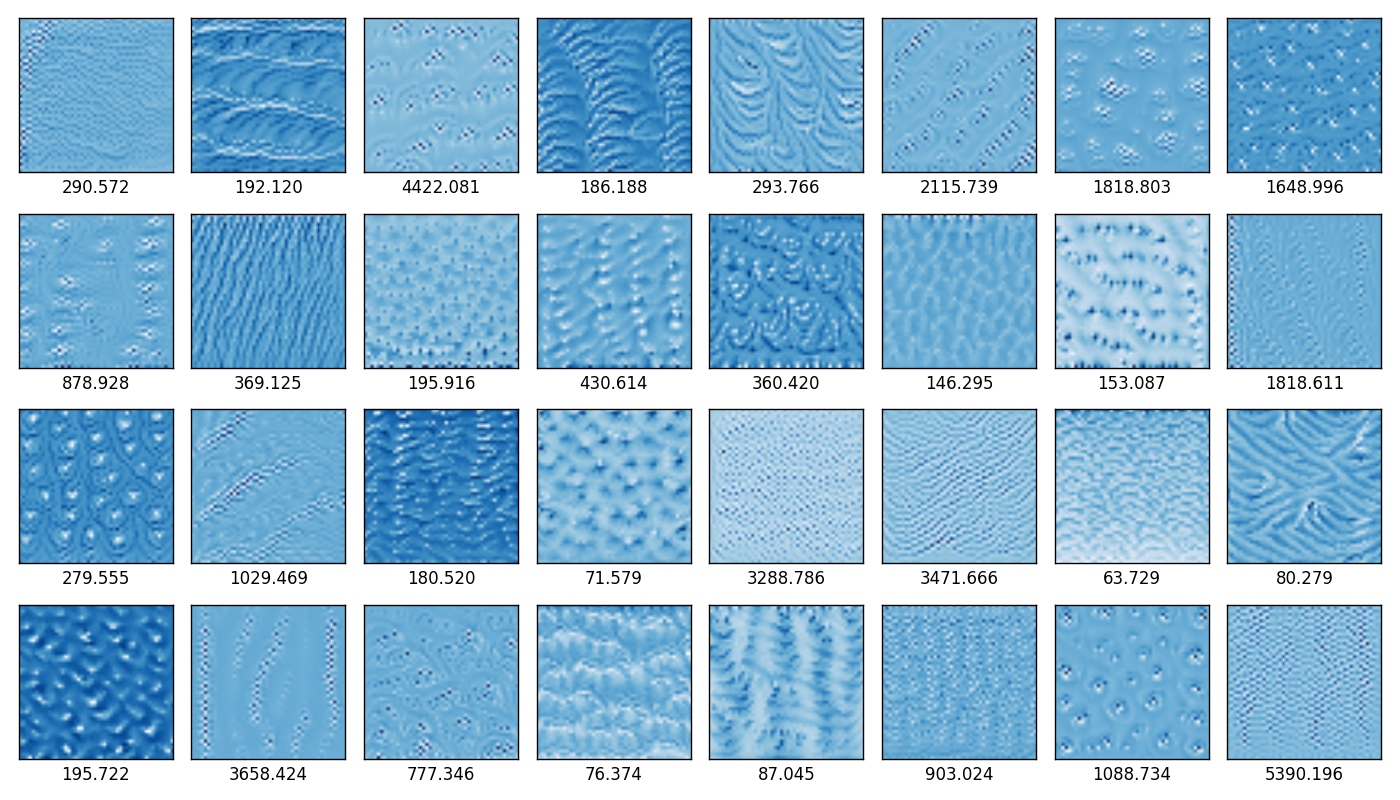
\includegraphics[width=\linewidth]{leaky_re_lu_4_e60.png}
      \caption{Layer: leaky relu 4 (epoch 60)}
      \label{fig:leaky_relu_4_e60}
    \end{subfigure}
    \caption{Gradient ascent from white noise}
    \label{fig:ga-white-noise}
  \end{figure}

  \par 而 Figure \ref{fig:filter-output},則是將 \texttt{train.csv} 當中的第 30 張圖片(屬於模型訓練時的 validation set)餵進去後,第一和第二層 Leaky ReLU Layer 輸出的結果。

  \begin{figure}[H]
    \begin{subfigure}[t]{0.5\textwidth}
      \centering
      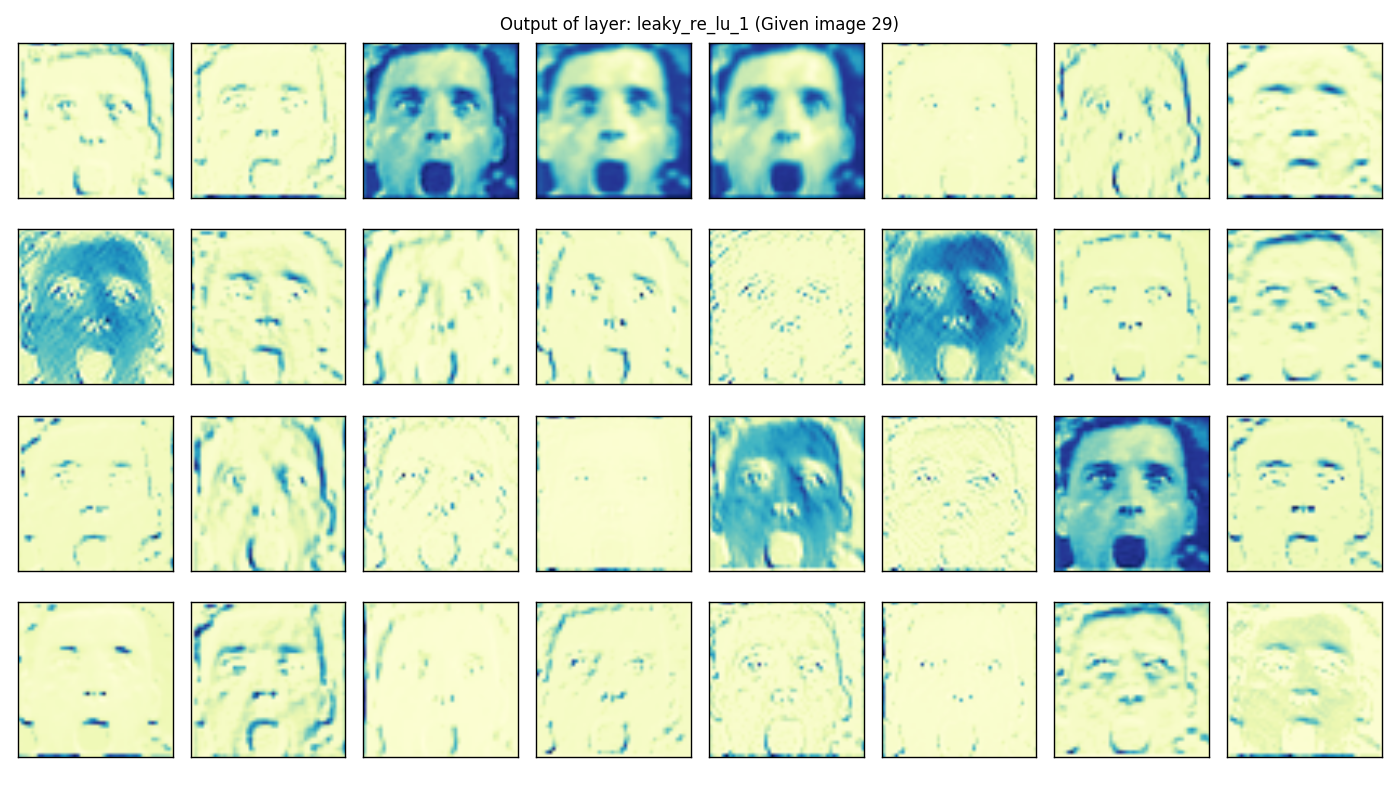
\includegraphics[width=\linewidth]{layer_leaky_re_lu_1.png}
      \caption{Layer: leaky relu 1}
      \label{fig:leaky_relu_1_output}
    \end{subfigure}
    \begin{subfigure}[t]{0.5\textwidth}
      \centering
      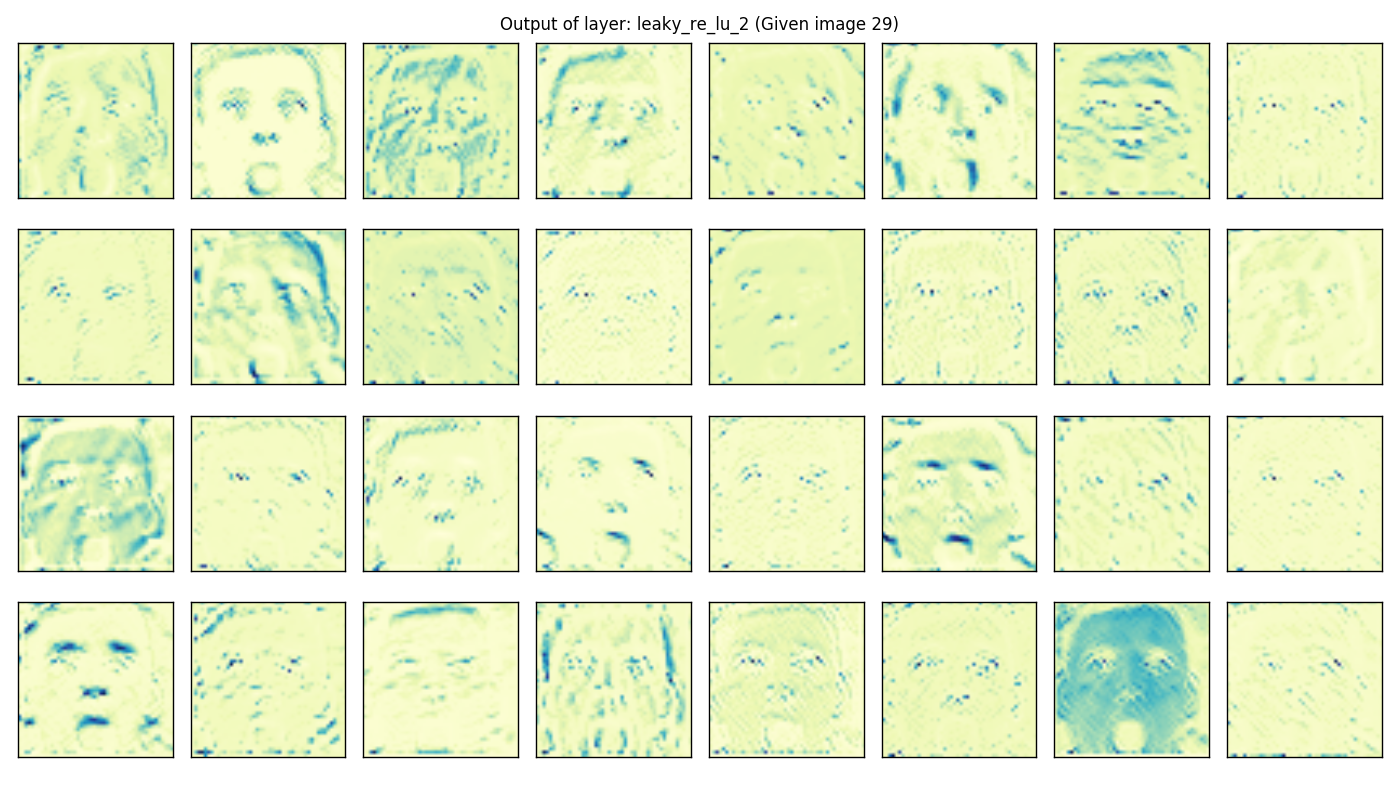
\includegraphics[width=\linewidth]{layer_leaky_re_lu_2.png}
      \caption{Layer: leaky relu 2}
      \label{fig:leaky_relu_2_output}
    \end{subfigure}
    \caption{Filter output (Image 29)}
    \label{fig:filter-output}
  \end{figure}

  \newpage

	\item[Bonus] (1\%) 從 training data 中移除部份 label,實做 semi-supervised learning。

	\item[Bonus] (1\%) 在 Problem 5 中,提供了3個 hint,可以嘗試實作及觀察(但也可以不限於 hint 所提到的方向,也可以自己去研究更多關於 CNN 細節的資料),並說明你做了些什麼?(完成1個:+0.4\%,完成2個:+0.7\%,完成3個:+1\%)

\end{enumerate}
\end{document}
